This chapter highlights the requirements of a digital back-end suited to a Q-Pix based readout implemented in a LArTPC design.

The first part of this chapter details the design problem which must solve data collection rates, total data aggretation, and hardware constraints for a successful deployment.
The Q-Pix readout~\ref{chap:qpix} relies on several key factors which promise possible improvements over a traditional MWPC readout: automatic calibration from quesicent background, an overall reduction in data collection, and simpler analysis and data reconstruction, to name a few.
However, this novel readout technique not only changes the front-end analog structure but also dramatically increases the number of digitization channels.
The increase of the number digital channels and required ASICs creates the need for a new digital-backend design.

The second part of this chapter describes a simulation framework which aims to parameterize the search for an optimal digital design.
We use a simulation framework to address these questions, since any sufficiently complicated design offers an intractible number of possible choices which can signficantly alter the performance (good or bad) of a detector.
The Q-Pix readout is no different.
A few examples of crucial design choices for the digital back-end are: the use of free-running local oscillators, the selection of an inter-ASIC communication protocol, the choice of inter-ASIC connections or routing profiles, and the buffer sizes of FIFOs to store charge-reset data.

The final part of this chapter summarizes the results of the simulations and provides, to the best of its ability, a description of the effects of the most important parameters determined from these results.
We use as inputs to the simulation the expected input charge from radiogenic background and beamline neutrino interaction over a DUNE-FD APA.
The goal of the next chapter~\ref{chap:qdb.tex} is to provide a hardware verification of the simulation results presented here.

The vast majority of the work presented in this chapter is my own individual work.

%%
\section{The Digital Back-end problem}

The main objectives of the digital back-end are to correctly measure the data presented to it by the analog front-end and ensure lossless transport of that data to disk.
More simply, the goals of the digital portion of the Q-Pix readout are to record and send data.
We note that the successful completion of these two objectives to be goal of these studies.

\subsection{The Basic Datum}

We begin with a discussion of the basic datum recorded and mention initial design choices at this interface.
The structure of this datum motivates the buffer widths and depths required to store the data at the local ASIC level as well as the protocol used to transfer this data between ASICs and eventually out of the detector.

The minimum data which needs to be recorded are the time, the relative location of the digitizing ASIC within the detector, plus any channels which were responsible for this reset.
Each of the number of bits assigned to recording these parameters are a design consideration.
We choose the number of bits for the timestamp ($N_{T}$) to be 32, which prevents frequency wrap-around based on a fast clock frequency (Equation~\ref{{eq:tloop}}).
We choose as the number of bits to assign a location ($N_{loc}$) to be 8, which provides a maximum possible number of unique positions before aggregation to be 256.
Next, since the number of pixels (required by analog front-end design) is 16 we choose this number as the number of bits to represent a ``mask'' ($N_{bits} = 16$).
We need to record all of the channels during each reset since it is technically possible (even if less likely) for multiple analog channels to provide a reset within the same clock window.

We calculate the minimum number of bits per datum to be:
\begin{equation}
  N_{bits} = N_{T} + N_{pix} + N_{loc} = 32 + 16 + 8 = 56
\end{equation}~\label{eq:nbits_datum}

Since buffer memory addresses and widths are normally characterized by powers of two, we can construct the basic datum size above the minimum number of bits provided by~\ref{eq:nbits_datum} to get $N_{datum} = 64$.
The remaining bits are useful for constructing different types of packets to be used by the digital ASICs for additional uses such as register configuration or to provide packet identification.

\subsection{Communication of the Datum}~\label{sec:comms}

There exist many asynchronous protocols of communication of digital information.
Most of the differences between protocols exist based on the number of connections between devices and whether or not one pin is allocated to share a clock, etc.

Our design considerations for this readout include reduction of SPF risk, low power, and minimal routing.
In part to these reasons, the design choice for communication relies on only two connections between ASICs with one defined as a data receiver (Rx) and the other as a data transmitter (Tx).
This choice of interface dramaticlaly limits a choice of possible protocols.
Here, we describe the difference between two that we tested: Universal Asynchronous receiver-transmitter (UART) and endeavor.
We discuss and test only these two protocols for simplicity and find it instructive to compare a proven and custom protocol (endeavor) against a very common one (UART).

The importance of choosing a correct protocl is to ensure lossless data transmission.
Since there are free running clocks, an asynchronous communication protocol is required.
The way to ensure that data can be moved between clocks of different speeds is to stretch the signal or to repeat bits.
The more the word is stretched in time, the larger the allowable difference in frequency between the two devices.
However, this lengthening can't proceed forever, obviously, otherwise words would become too long.

It is another important design consideration in this design to ensure that transactions do not take too long.
Unnecessarily long transactions which take up more clock cycles use more power and increase the noise risk to leak to the analog front-end.


%% appendix??
\subsubsection{UART}
This common protocol is typically stable between devices with a maximum difference of clock frequency to be 10\%.

%% appendix??
\subsubsection{Endeavor}
This protocol is slower than UART, but allows for double the frequency difference: $\approx$ 20\%.

%% This section should reference how Q-Pix fits into a DUNE APA as a design goal
\section{Constraining the Digital-Backend Design}

Section~\ref{sec:qpix_apa} describes in detail how a Q-Pix based hardware readout architecture could fit within a single DUNE-APA.
Here we extend this discussion and use those constraints as the starting point for a search for a solution to the digital back-end architecture.
The first problem to solve is how to aggregate the all timestamp data supplied by the large number of channels within a DUNE-FD APA.

A Q-Pix architecture would likely use either a high-performance FPGA or a custom ASIC to aggregate the large number of $(\mathcal{O}(10^{7})$ channels .
The number of aggregated digital channels determines the required capabilities of the aggregator node and the selection of an FPGA or ASIC.
Since each additional aggregator node represents an additional SPF risk, our design goal suggests that the optimal configuration is one that produces the least number of aggregator nodes.
Therefore, the goal is to design a routing architecture as big as possible for each data aggregator node which still allows for accurate timing calibration and lossless data acquisition.

However, as one increases the number of digital channels per aggregator node one also increases the amount of local oscillators per aggregator, each of which must be calibrated.
Additionally, since each digital channel requires extra communication time (as discussed in section~\ref{sec:comms}) the introduction of more channels negatively affects the precision of timing calibrations and increases SPF risk.
We consider then that an optimal number of digital channels per aggregator node is one that maximizes the number of digital channels but still maintains the required timing calibration~(Sec.~\ref{sec:background}) and transmits lossless data.

We refer to the total number of digital channels collected from one pathway to an aggregator as a tile.
In a fully realized design an aggregator might in fact be responsible for multiple tiles, which need not necessarily be the same size.
The parameteriziation of an aggregator node is completely determined by the composition of tiles it is connected to.
Then, a parameteriziation of the data requirements imposed by each tile can be extended to describe the requirements of the aggregator node.
Finally, we reach the conclusion that the required parameterization of the back-end system relies on the parameterization of the tile.

The construction of a tile is the inter-connections between digital channels.
The LArTPC design also suggests that each digital channel have a maximum of four connections since the collection of charge happens on a flat two-dimmensional anode plane.
Therefore, a two-dimensional routing requires at least two independent communication channels, which if we require the digital channels to be symmetric (they can communicate in both directions along each axis), the minimum number of connection channels is four.
We use this number as a starting point for the digital channel design.
Also, four connections per channel immediately creates a rectangular connection structure for a tile.

% once aggregator is selected, hardware can be parameterized
We note here that in order to meet other physical design requirements to fit into a pre-existing APA frame, the capability of the aggregator nodes could be increased to be responsible for more tiles, which would reduce the cable and hardware engineering considerations.
However, further consideration here is beyond the scope of this work.


% tile connection methods
\subsection{Tile Routing Considerations}

A tile is a rectangular composition of digital channels which must a path to all digital channels and send lossless data to the aggregator.
Since there is one connection between a tile and the aggregator, there is one special node within the tile that connects to the aggregator.
This special node we refer to as the ``base-node'' as all data and instruction commands, regardless of routing, must pass through this node.
The symmetry of the rectangular tile allows any corner node to be the base node, and we choose the upper-left to define a convention.

We do not consider possible configurations where an aggregator might be connected to a digital channel within a tile since we require that all channels are identical and fully connected.
Further, we address that we discuss why we do not consider base-nodes placed on the outter edge of a tile, but not at the corners more generally in section~\ref{sec:base_node}.
Briefly, base-nodes which are along the outter edge of a FCT but not at the corners simply contain two sub-graphs of FCT with a base-node along the edge.
Therefore, an analysis of the constraints of a FCT with corner base-nodes can be mapped to an analysis of FCT with edge base-nodes.

Here we introduce a particular representation (based on graph-theory) for a tile which is useful for simplifying simulations and for analyzing particular routing configurations.
The most general tile configuration occurs when we assume that all adjacent nodes within the tile are connected; this creates what we refer to as a ``fully connected tile'' (FCT).
An example of a FCT is shown in Figure~\ref{fc_tile}.
Any particular choice of an effective routing must then be a subset of this fully connected version.

\begin{figure}[]
\centering
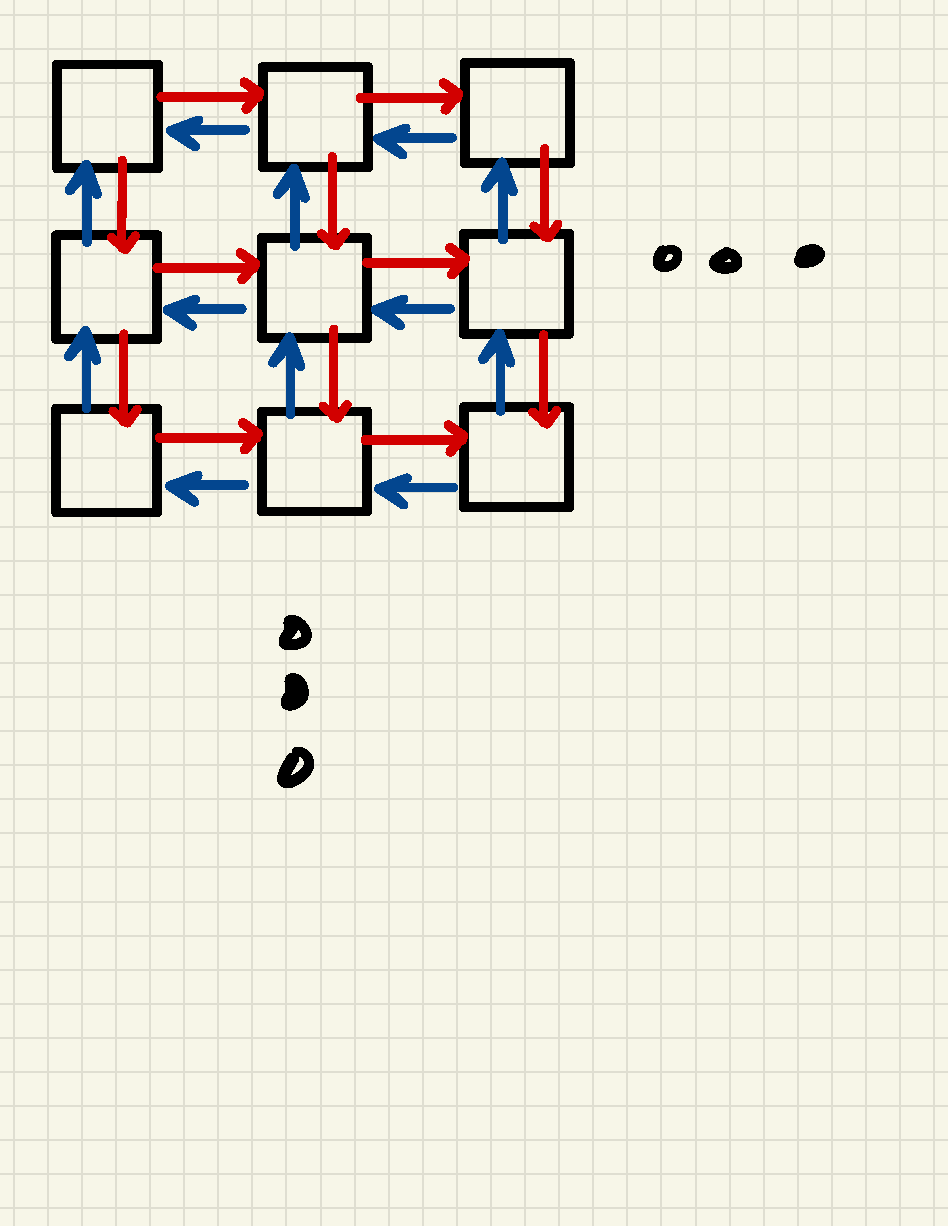
\includegraphics[width=\textwidth]{images/Notes.pdf}
\caption{Example of the fully connected routing configuration for a tile (FCT). Each Node represents a digital channel which must be aggregated, and the red and blue connections distinguish directions of communication. The red connection lines indicate pathways away from the base node, whereas the blue lines represent connection paths towards the base-node in the upper-left.}
\end{figure}~\label{fig:fc_tile}

To elaborate on the adjacency matrix of the FCT we consider an $2\times 3$ tile.
A $2\times 3$ tile has six total nodes, where we consider the upper-left most node to be the base node.
Then, the unweighted adjacency matrix has dimensions $6\times6$ of the form:
\begin{equation}
M =
 \begin{pmatrix}
 0 & 1 & 0 & 1 & 0 & 0 \\
 1 & 0 & 1 & 0 & 1 & 0 \\
 0 & 1 & 0 & 0 & 0 & 1 \\
 1 & 0 & 0 & 0 & 1 & 0 \\
 0 & 1 & 0 & 1 & 0 & 1 \\
 0 & 0 & 1 & 0 & 1 & 0 \\
 \end{pmatrix}
\end{equation}~\label{eq:adjacency_matr}

Where each non-zero value of $M_{ij}$ represents a connection between nodes $i$ and $j$.
As an unweighted, undirected graph this is a symmetric matrix.

In practice each digital channel within a tile is actually controlled by a unique, free-running oscillator.
Therefore, we can define the length of each edge between nodes as the length of time to send of a packet of data between two nodes ($T_{i\rightarrow j}$).
With this we can extend the model the adjacency matrix as a weighted and directed graph if we recognize that the non-zero elements of $M_{ij}$ become $T_{i\rightarrow j}$, or the length of time it takes for the $i^{th}$ local oscillator to transmit a packet to node $j$.

We can generalize this matrix in terms of an arbitrary number of rows ($r$) and columns ($c$).
We define a convention of numbering nodes within the tile in terms of increasing column number followed by increasing row number.
With this convention we obtain the general adjacency matrix with values defined by:
\begin{equation}
  M_{ij} = T_{i\rightarrow j}(\delta_{i,j=i\pm 1} + \delta_{i,j=i\pm r})
\end{equation}~\label{eq:adjacency_comp}

The length between the nodes represets the time it takes for a packet to transact from one node to the next.
This is determined by both the number of bits to be sent in the communication protocol ($N_{bits}$ and the frequency of the local oscillator ($f_{i}$).
We note that the receiving local oscillator also affects the true transaction time up to a single clock cycle.
However, since the transaction time of a packet is much larger than a single clock cycle ($N_{bits} \simeq \mathcal{O}10^{2} \gg 1$), we can approximate: $T_{i\rightarrow j} \approx T_{i} = N_{bits}/f_{i}$.

This representation is also useful to model certain SPF where a node becomes inactive.
Dead or inactive nodes are ones in which all of their connections are effectively disconnected.
This is equivalent to setting their transaction lengths to zero: $T_{SPF} = 0$.

We comment that although it is possible to construct tiles where more than one node connects to the aggregator, we observe that this configuration simply produces two effective tiles.
These distinct tiles then are the data paths which are unique to each base-node.
In this graphical representation a packet of data can follow one, and only one path from the origin node to the base-node unless there was duplication of packets.
We emphatically avoid designs which might depend on data duplication for reduncancy; these two base-nodes are in unconnected graphs.

Additionally, it is possible to connect non-rectangular tiles, but these tiles are effectively a larger rectangular tile with disconnected nodes to produce the desired shape.
Since every node is designed to be robust in the full version, it will be be robust in the subset.

We can apply this same argument to base-nodes which do not lie at the corners of the rectangular tile.
In the case where the base-node is selected along the edge
Therefore, we conclude that the analysis of the tile with the above adjacency matrix and a selection of the base-node at the corner of a rectangular corner provides the basis problem to the tile configuration.

\subsubsection{Minimize Connections Count}~\label{sec:min_conn}

\subsubsection{Minimize Communication Delay}~\label{sec:min_comm}

\subsubsection{Broadcasts to avoid SPF}~\label{sec:broadcast}

In order to protect against SPF we consider a design which uses the FCT.
A FCT allows searches to probe all possible paths to any node via a ``broadcast'' produced from packets sent by the aggregator to the base-node.
Therefore the broadcast algorithm can be represented by a complete circuit which begins at the base-node and proceeds to a target node with no repeated nodes until the target node is reached.
The backward path is then completed in reverse by following the edges (connections) between each node until arriving finally again at the base-node.

In the event that a particular node becomes inactive it will ``block'' data comming from the nodes along its path.
In this case, there must be some sort of ``broadcast'' originating from the base-node that would allow information tranverse regardless of the effective routing path.

Since SPF, by definition, can occur on any node the most robust connection scheme is the full connection.
A full connection

\subsection{The Edge Base-node}~\label{sec:base_node}

We discuss here the case of a FCT with an edge base node.
An edge base node (EBN) is a digital channel that connects to the aggregator and to three other digital channels within a tile.
Like before, this base-node must provide a path to all digital channels within the tile.
In this configuration the adjacency matrix is the same as shown in~\ref{eq:adjacency_comp}.

Also as before we wish to inspect different routing scenarios for a tile of a given square dimension of $R$ rows and $C$ columns.
We can proceed by dividing the FCT graph into two subgraphs, $S1$ and $S2$, where $S1$ represets the rectangular section of the graph below and to the left of the EBN, while $S2$ are the remaining channels.

We identify that while the number of columns ($C$) in tile is equal to both subgraphs, the total number of rows $R$ of the tile is equal to the sum of the rows from these two subgraphs: $R = R_{1} + R_{2}$.



%%
\section{Physical Simulation Studies}

%%
\section{Background Rates and Calibration}

sources of backgrounds are taken from \citep{DUNE-FD_TDRv4:Abi_2020}

\section{Supernova Studies}

Work has been done to understand how a Q-Pix based DUNE-FD would measure core collapse supernovae \citep{qpix:shion}.

Simulation studies which involved particle interactions were based on Geant4 \citep{geant4:AGOSTINELLI2003250}.


\section{Looking for Hadron Decay}

\section{Neutrino Beam High Energy Studies}

\section{Summary and Further Studies}
